\documentclass[aspectratio=169]{beamer}
\usefonttheme[onlymath]{serif}
\usepackage[brazilian]{babel}

\mode<presentation>
{
  \usetheme{Darmstadt}     % or try Darmstadt, Madrid, Warsaw, ...
  \usecolortheme{beaver} % or try albatross, beaver, crane, ...
  \usefonttheme{default}  % or try serif, structurebold, ...
  \setbeamertemplate{navigation symbols}{}
  \setbeamertemplate{caption}[numbered]
  \setbeamertemplate{headline}{}
}

%%%%%%%%%%%%%%%%%%%%%%%%%%%%%%%%%%%%%%%%%%%%%%%%%%%%%%%%%

\usepackage{mathtools}
%\usepackage{amsthm}
\usepackage{amsmath}
%\usepackage{nccmath}
\usepackage{amssymb}
%\usepackage{amsfonts}
\usepackage{physics}
%\usepackage{dsfont}
%\usepackage{mathrsfs}
%\usepackage{slashed}    % Feynman slash notation, requires LuaLaTeX
%\usepackage[compat=1.1.0]{tikz-feynman}   % Feynman diagrams

%\usepackage{titling}
\usepackage{indentfirst}
%\usepackage[titletoc,title]{appendix}
%\renewcommand\appendixname{Apêndice}

\usepackage{bm}
%\usepackage{xcolor}
%\usepackage[dvipsnames]{xcolor}
\usepackage{cancel}

%\usepackage{xurl}
\usepackage{hyperref}
\usepackage{cite}

\usepackage{float}
\usepackage{graphicx}
\usepackage{tikz}
\usepackage{caption}
\usepackage{subcaption}

%%%%%%%%%%%%%%%%%%%%%%%%%%%%%%%%%%%%%%%%%%%%%%%%%%%

\newcommand{\eps}{\epsilon}
\newcommand{\vphi}{\varphi}
\newcommand{\cte}{\text{cte}}

\newcommand{\N}{\mathbb{N}}
\newcommand{\Z}{\mathbb{Z}}
\newcommand{\Q}{\mathbb{Q}}
\newcommand{\R}{\vb{R}}
\newcommand{\C}{\mathbb{C}}
\renewcommand{\S}{\vb{S}}
%\renewcommand{\H}{\s{H}}

\renewcommand{\a}{\vb{a}}
\renewcommand{\b}{\vb{b}}
\renewcommand{\d}{\dagger}
\newcommand{\up}{\uparrow}
\newcommand{\down}{\downarrow}
\newcommand{\hc}{\text{h.c.}}

\newcommand{\0}{\vb{0}}
\newcommand{\1}{\mathds{1}}
\newcommand{\E}{\vb{E}}
\newcommand{\B}{\vb{B}}
\renewcommand{\v}{\vb{v}}
\renewcommand{\r}{\vb{r}}
\renewcommand{\k}{\vb{k}}
\newcommand{\p}{\vb{p}}
\newcommand{\q}{\vb{q}}
\newcommand{\F}{\vb{F}}
\newcommand{\A}{\vb{A}}
\newcommand{\J}{\vb{J}}

\newcommand{\s}{\sigma}
\newcommand{\nn}[2]{\left\langle #1 , #2 \right\rangle}
\newcommand{\cc}[1]{\overline{#1}}
\newcommand{\Eval}[3]{\eval{\left( #1 \right)}_{#2}^{#3}}

\newcommand{\unit}[1]{\; \mathrm{#1}}

\newcommand{\n}{\medskip}
\newcommand{\e}{\quad \mathrm{e} \quad}
\newcommand{\ou}{\quad \mathrm{ou} \quad}
\newcommand{\virg}{\, , \;}
\newcommand{\ptodo}{\forall \,}
\renewcommand{\implies}{\; \Rightarrow \;}
%\newcommand{\eqname}[1]{\tag*{#1}} % Tag equation with name


%%%%%%%%%%%%%%%%%%%%%%%%%%%%%%%%%%%%%%%%%%%%%%%%%%%%%%%%%

\title[Exercício 4, Lista 1 - Física do Estado Sólido I]{\LARGE{Exercício 4, Lista 1 - Física do Estado Sólido I}}
\author[Mateus Marques]{\large{Mateus Marques}}
\institute[]{\small{Instituto de Física da Universidade de São Paulo}}
\titlegraphic{
\includegraphics[height=1.5cm]{fig/ifusp.png}}

\begin{document}

\begin{frame}
  \titlepage
\end{frame}

%\section{Introdução}

\begin{frame}{(a) Rede recíproca}

Dada uma rede de Bravais, sua rede recíproca é definida pelos vetores $\vb{G}$ tais que $e^{i \vb{G} \vdot \vb{R}} = 1$, para todos os vetores $\vb{R}$ na rede de Bravais. Uma onda plana $e^{i \k \vdot \r}$ tem periodicidade da rede de Bravais se, e somente se, $\k$ pertencer à rede recíproca.

\n

Sendo $\a_i$ os vetores primitivos da rede de Bravais, a condição para os vetores primitivos $\b_j$ da rede recíproca se traduz em
\begin{equation} \label{eq:b-cond}
\a_i \vdot \b_j = 2\pi \delta_{ij}
\end{equation}

\n

Sendo $\Omega = \abs{\a_1 \vdot (\a_2 \times \a_3)}$ o volume da célula unitária da rede de Bravais, os vetores $\b_1 = \frac{2\pi}{\Omega} (\a_2 \times \a_3)$, $\b_2 = \frac{2\pi}{\Omega} (\a_3 \times \a_1)$ e $\b_3 = \frac{2\pi}{\Omega} (\a_1 \times \a_2)$ satisfazem a condição (\ref{eq:b-cond}).

\n

Neste exercício, calcularemos os vetores primitivos da rede recíproca para as redes
\begin{itemize}
\item Quadrada 2D;
\item Hexagonal 2D;
\item Cúbica;
\item Cúbica de corpo centrado (BCC).
\end{itemize}

\end{frame}


%%%%%%%%%%%%%%%%%%%%%%%%%%%%%%%%%%%%%%%%%%%%%%%%%%%%%%%%%


\begin{frame}{Rede quadrada}

$\a_1 = a(1,0,0)$, $\a_2 = a(0,1,0)$, $\a_3 = (0,0,1)$, $\Omega = \abs{\a_1 \vdot (\a_2 \times \a_3)} = a^2$.

\n

Note que a rede quadrada é 2D, mas podemos utilizar um vetor primitivo ``artificial'' $\a_3 = (0,0,1)$ somente para fazer o cálculo de $\b_1$ e $\b_2$ através das expressões mencionadas.
$$
\b_1 = \frac{2\pi}{\Omega} \, \a_2 \times \a_3 = \frac{2\pi}{a} \, \vu{y} \times \vu{z} = \frac{2\pi}{a} \vu{x} = \frac{2\pi}{a} (1, 0).
$$
$$
\b_2 = \frac{2\pi}{\Omega} \, \a_3 \times \a_1 = \frac{2\pi}{a} \, \vu{z} \times \vu{x} = \frac{2\pi}{a} \vu{y} = \frac{2\pi}{a} (0, 1).
$$

Assim, a recíproca da rede quadrada também é uma rede quadrada, mas com distância de rede $\frac{2\pi}{a}$.

\end{frame}


%%%%%%%%%%%%%%%%%%%%%%%%%%%%%%%%%%%%%%%%%%%%%%%%%%%%%%%%%


\begin{frame}{Simetrias da rede quadrada}

\begin{figure}[H]
\centering
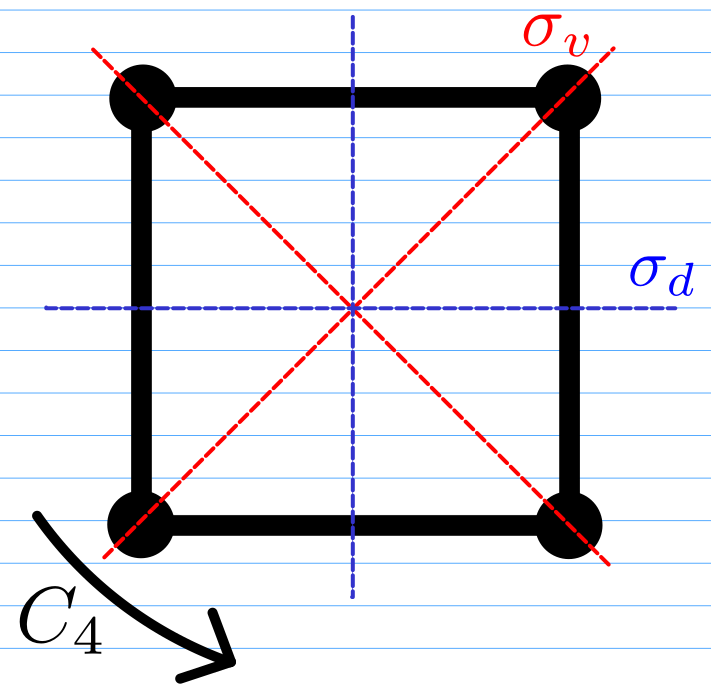
\includegraphics[width=0.3\linewidth]{fig/symm_square.png}
\caption{Célula unitária da rede quadrada e suas simetrias.}
\label{fig:symm_square}
\end{figure}

\begin{itemize}
\item Rotações $C_4$ (por $90^\circ$ no eixo $z$).
\n
\item Reflexões $\sigma_h$, $\sigma_v$ e $\sigma_d$.
\n
\item Inversão.
\end{itemize}

\end{frame}


%%%%%%%%%%%%%%%%%%%%%%%%%%%%%%%%%%%%%%%%%%%%%%%%%%%%%%%%%


\begin{frame}{Rede hexagonal}

A escolha dos vetores primitivos de uma rede de Bravais não é única. Para a rede hexagonal, uma escolha natural é de dois vetores de mesmo módulo que formam um ângulo de $60^\circ$.

\begin{figure}[H]
\centering
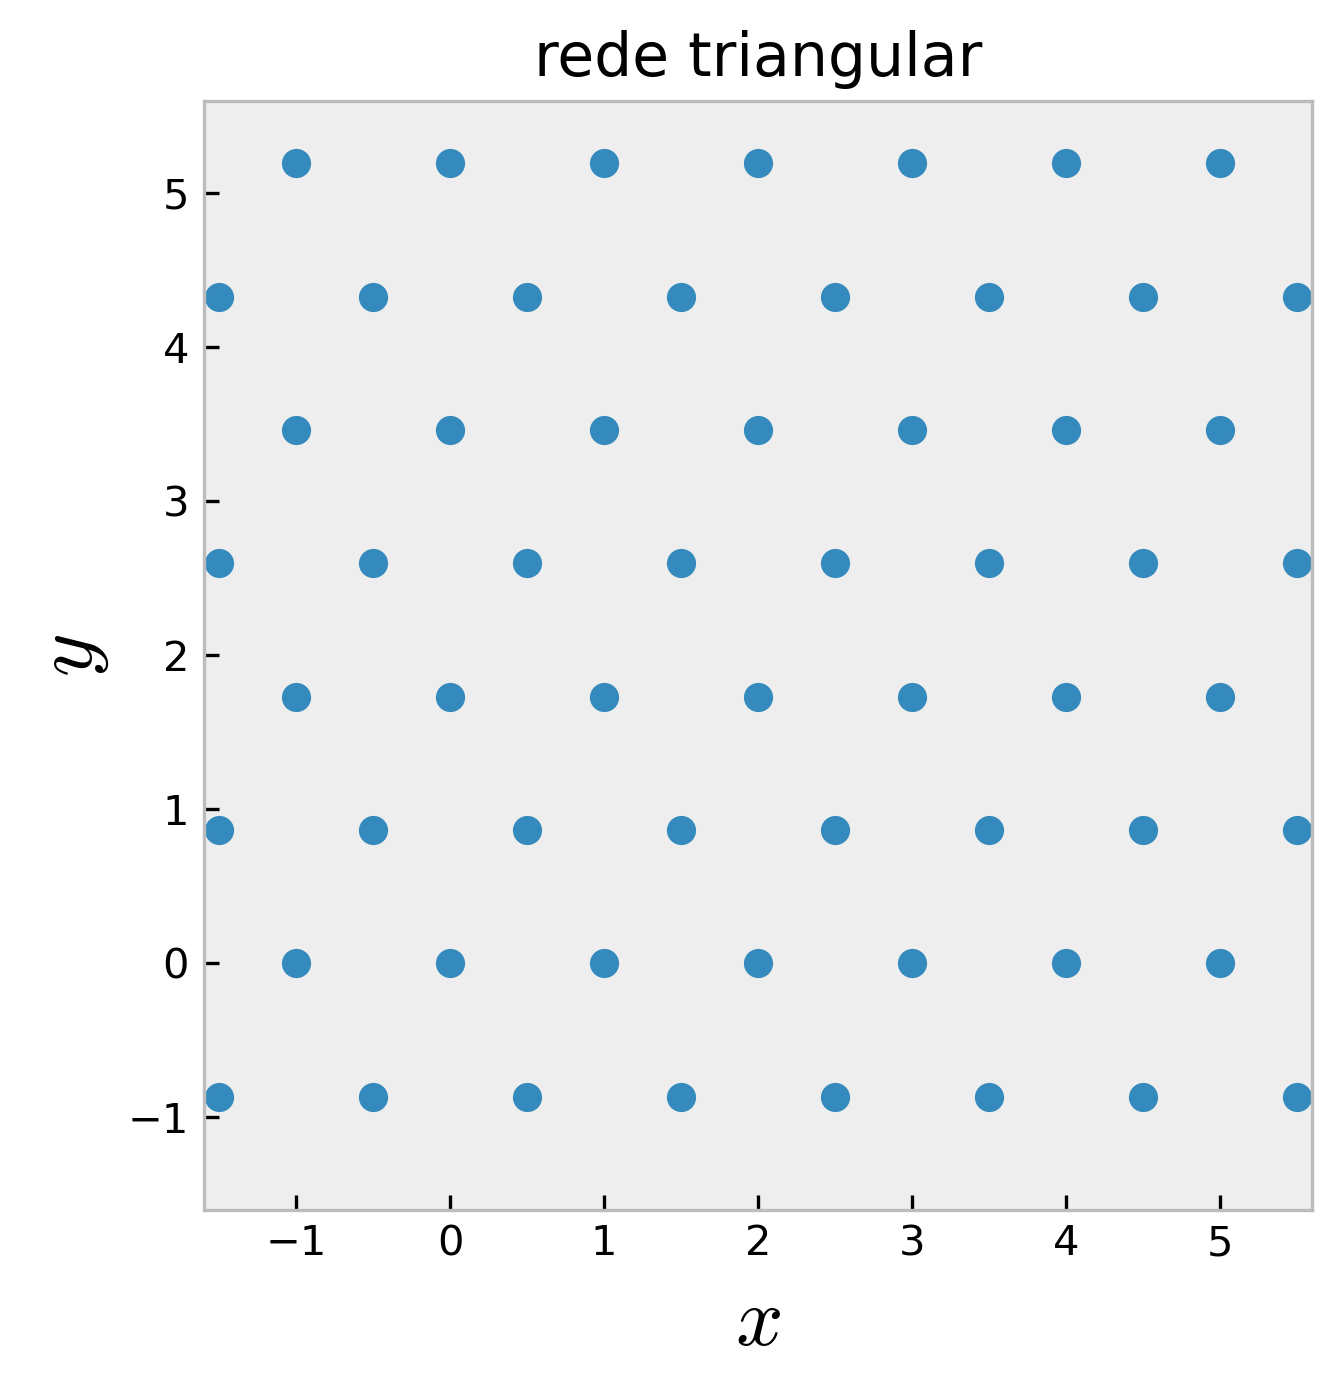
\includegraphics[width=0.35\linewidth]{fig/lattice_triang.png}
\caption{Rede hexagonal (triangular).}
\label{fig:lat-triang}
\end{figure}

\end{frame}


%%%%%%%%%%%%%%%%%%%%%%%%%%%%%%%%%%%%%%%%%%%%%%%%%%%%%%%%%


\begin{frame}{Rede hexagonal}

$\a_1 = a(1,0,0)$, $\a_2 = a\qty(\frac{1}{2},\frac{\sqrt{3}}{2},0)$, $\a_3 = (0,0,1)$, $\Omega = \abs{\a_1 \vdot (\a_2 \times \a_3)} = \frac{a^2 \sqrt{3}}{2}$.
$$
\b_1 = \frac{2\pi}{\Omega} \, \a_2 \times \a_3 =
\frac{4\pi}{a \sqrt{3}}
\begin{vmatrix}
\vu{x} & \vu{y} & \vu{z} \\
\frac{1}{2} & \frac{\sqrt{3}}{2} & 0 \\
0 & 0 & 1 \\
\end{vmatrix}
=
\frac{4\pi}{a \sqrt{3}} \qty(\frac{\sqrt{3}}{2} \vu{x} - \frac{1}{2} \vu{y}).
$$
$$
\b_2 = \frac{2\pi}{\Omega} \, \a_3 \times \a_1 =
\frac{4\pi}{a \sqrt{3}}
\begin{vmatrix}
\vu{x} & \vu{y} & \vu{z} \\
0 & 0 & 1 \\
1 & 0 & 0 \\
\end{vmatrix}
= \frac{4\pi}{a\sqrt{3}} \vu{y}.
$$

O ângulo entre $\b_1$ e $\b_2$ é $\cos\theta = \frac{\b_1 \vdot \b_2}{\abs{\b_1}\,\abs{\b_2}} = -\frac{1}{2} \implies \theta = 120^\circ$. Como o ângulo é $120^\circ$, a rede recíproca também forma uma rede hexagonal.

\end{frame}


%%%%%%%%%%%%%%%%%%%%%%%%%%%%%%%%%%%%%%%%%%%%%%%%%%%%%%%%%


\begin{frame}{Rede hexagonal}

A Figura \ref{fig:hex_bz} mostra os vetores primitivos da rede recíproca e a zona de Brillouin.

\begin{figure}[H]
\centering
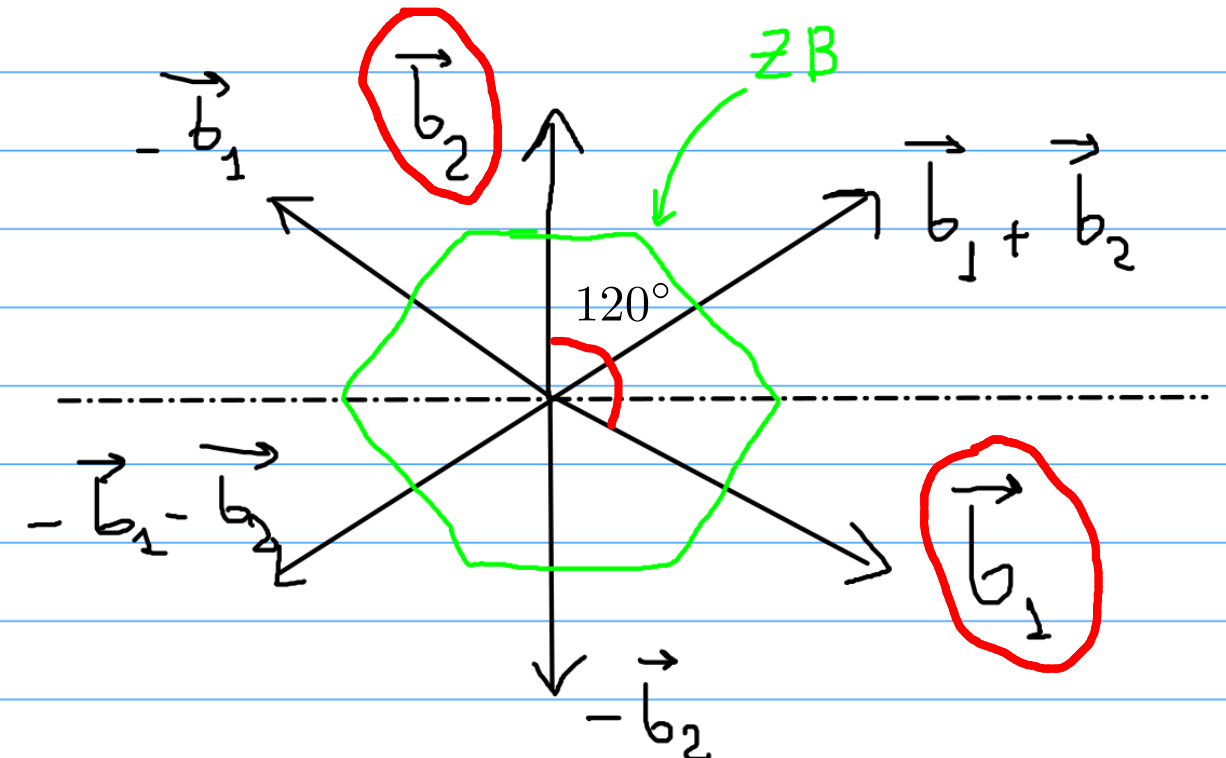
\includegraphics[width=0.65\linewidth]{fig/hex_bz}
\caption{Vetores primitivos da rede recíproca da rede hexagonal e a zona de Brillouin.}
\label{fig:hex_bz}
\end{figure}

\end{frame}


%%%%%%%%%%%%%%%%%%%%%%%%%%%%%%%%%%%%%%%%%%%%%%%%%%%%%%%%%


\begin{frame}{Simetrias da rede hexagonal}

\begin{figure}[H]
\centering
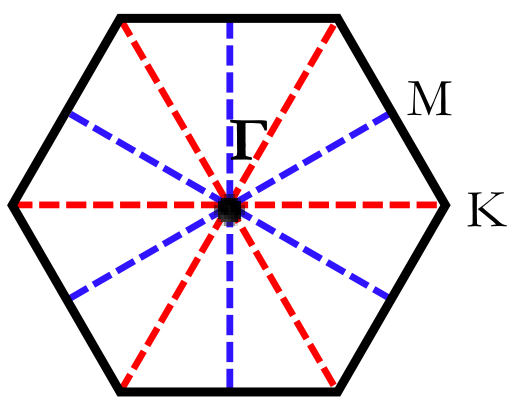
\includegraphics[width=0.3\linewidth]{fig/symm_hexago.png}
\caption{Célula unitária da rede hexagonal e suas simetrias. As linhas pontilhadas vermelhas indicam as reflexões $\textcolor{red}{\sigma_v}$ e as azuis $\textcolor{blue}{\sigma_d}$.}
\label{fig:symm_hexago}
\end{figure}

\begin{itemize}
\item Rotações $C_6$ (por $60^\circ$ no eixo $z$).
\n
\item Reflexões $\sigma_h$, $\sigma_v$ e $\sigma_d$.
\n
\item Inversão.
\end{itemize}

\end{frame}


%%%%%%%%%%%%%%%%%%%%%%%%%%%%%%%%%%%%%%%%%%%%%%%%%%%%%%%%%


\begin{frame}{Rede cúbica}

$\a_1 = a \vu{x}$, $\a_2 = a\vu{y}$ e $\a_3 = a\vu{z}$, $\Omega = a^3$.

\n

Analogamente à rede quadrada, os vetores primitivos da rede cúbica são calculados facilmente como:
$$
\b_1 = \frac{2\pi}{a} \vu{x}, \quad \b_2 = \frac{2\pi}{a} \vu{y}, \quad \b_3 = \frac{2\pi}{a} \vu{z}.
$$

Assim, sua rede recíproca também é uma rede cúbica, só que com distância de rede $\frac{2\pi}{a}$.

\end{frame}


%%%%%%%%%%%%%%%%%%%%%%%%%%%%%%%%%%%%%%%%%%%%%%%%%%%%%%%%%


\begin{frame}{Simetrias da rede cúbica}

\begin{figure}[H]
\centering
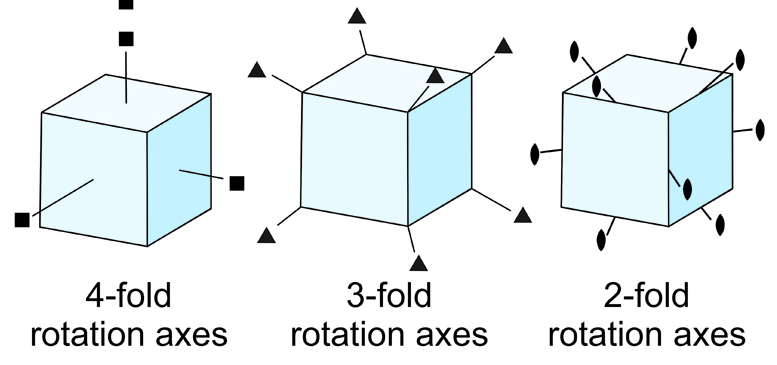
\includegraphics[width=0.6\linewidth]{fig/rot_cubic.png}
\caption{Eixos de rotação da rede cúbica.}
\label{fig:rot_cubic}
\end{figure}


\begin{itemize}
\item Rotações $C_4$ (nos eixos $x, y, z$).
\item Rotações $C_3$ (eixos das diagonais).
\item Rotações $C_2$ (eixos que passam pelos pontos médios das arestas).
\end{itemize}

\end{frame}


%%%%%%%%%%%%%%%%%%%%%%%%%%%%%%%%%%%%%%%%%%%%%%%%%%%%%%%%%


\begin{frame}{Simetrias da rede cúbica}

\begin{figure}[H]
\centering
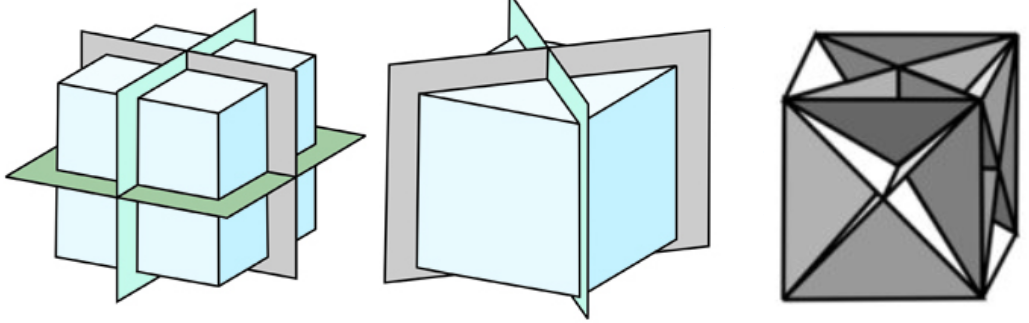
\includegraphics[width=0.6\linewidth]{fig/reflex_cubic.png}
\caption{Planos de reflexão da rede cúbica.}
\label{fig:reflex_cubic}
\end{figure}


\begin{itemize}
\item Reflexões (na Figura \ref{fig:reflex_cubic}).
\n
\item Identidade e Inversão.
\end{itemize}

\end{frame}


%%%%%%%%%%%%%%%%%%%%%%%%%%%%%%%%%%%%%%%%%%%%%%%%%%%%%%%%%


\begin{frame}{Rede BCC}

Rede cúbica de corpo centrado: Nesse caso consideraremos os vetores primitivos desenhados na Figura \ref{fig:bcc}:
\begin{figure}[H]
\centering
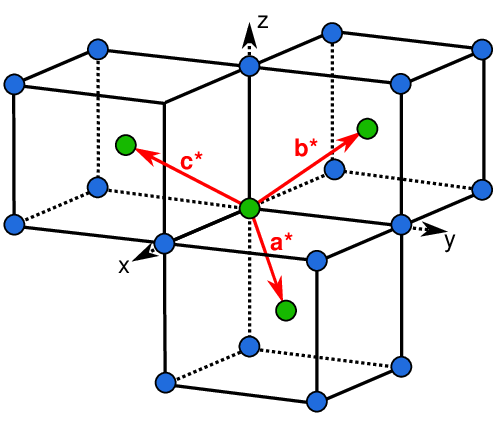
\includegraphics[width=0.35\linewidth]{fig/bcc.png}
\caption{Vetores primitivos da rede BCC. ($\a^{*} \equiv \a_1, \b^{*} \equiv \a_2, \vb{c}^{*} \equiv \a_3$).}
\label{fig:bcc}
\end{figure}

$\a_1 = \frac{a}{\sqrt{3}}(1, 1, -1)$, $\a_2 = \frac{a}{\sqrt{3}}(-1, 1, 1)$ e $\a_3 = \frac{a}{\sqrt{3}}(1, -1, 1)$. (Os vetores têm norma $a$).

\end{frame}


%%%%%%%%%%%%%%%%%%%%%%%%%%%%%%%%%%%%%%%%%%%%%%%%%%%%%%%%%


\begin{frame}{Rede BCC}

Temos então
$$
\Omega = \abs{\a_1 \vdot (\a_2 \times \a_3)} =
\frac{a^3}{3\sqrt{3}}
\begin{vmatrix}
1 & 1 & -1 \\
-1 & 1 & 1 \\
1 & -1 & 1 \\
\end{vmatrix}
=
\frac{4a^3}{3\sqrt{3}}.
$$
$$
\b_1 = \frac{2\pi}{\Omega}
\begin{vmatrix}
\vu{x} & \vu{y} & \vu{z} \\
-1 & 1 & 1 \\
1 & -1 & 1 \\
\end{vmatrix}
=
\frac{3\pi\sqrt{3}}{2a^3} (2\vu{x} + 2\vu{y}) = \frac{3\pi\sqrt{3}}{a^3} (1, 1, 0).
$$
$$
\b_2 = \frac{2\pi}{\Omega}
\begin{vmatrix}
\vu{x} & \vu{y} & \vu{z} \\
1 & -1 & 1 \\
1 & 1 & -1 \\
\end{vmatrix}
=
\frac{3\pi\sqrt{3}}{2a^3} (2\vu{y} + 2\vu{z}) = \frac{3\pi\sqrt{3}}{a^3} (0, 1, 1).
$$
$$
\b_3 = \frac{2\pi}{\Omega}
\begin{vmatrix}
\vu{x} & \vu{y} & \vu{z} \\
1 & 1 & -1 \\
-1 & 1 & 1 \\
\end{vmatrix}
=
\frac{3\pi\sqrt{3}}{2a^3} (2\vu{x} + 2\vu{z}) = \frac{3\pi\sqrt{3}}{a^3} (1, 0, 1).
$$

\end{frame}


%%%%%%%%%%%%%%%%%%%%%%%%%%%%%%%%%%%%%%%%%%%%%%%%%%%%%%%%%


\begin{frame}{Rede recíproca da BCC é a FCC}

Perceba que os vetores obtidos formam uma rede de face centrada (FCC):
\begin{figure}[H]
\centering
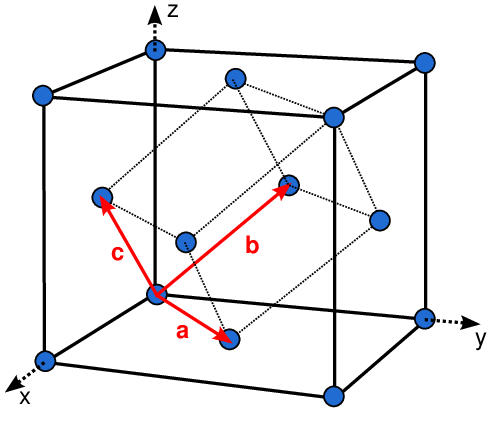
\includegraphics[width=0.4\linewidth]{fig/fcc.png}
\caption{Rede FCC e vetores primitivos. ($\a \equiv \b_1, \b \equiv \b_2, \vb{c} \equiv \b_3$).}
\label{fig:fcc}
\end{figure}

\end{frame}


%%%%%%%%%%%%%%%%%%%%%%%%%%%%%%%%%%%%%%%%%%%%%%%%%%%%%%%%%


\begin{frame}{Simetrias da rede FCC}

\begin{figure}[H]
\centering
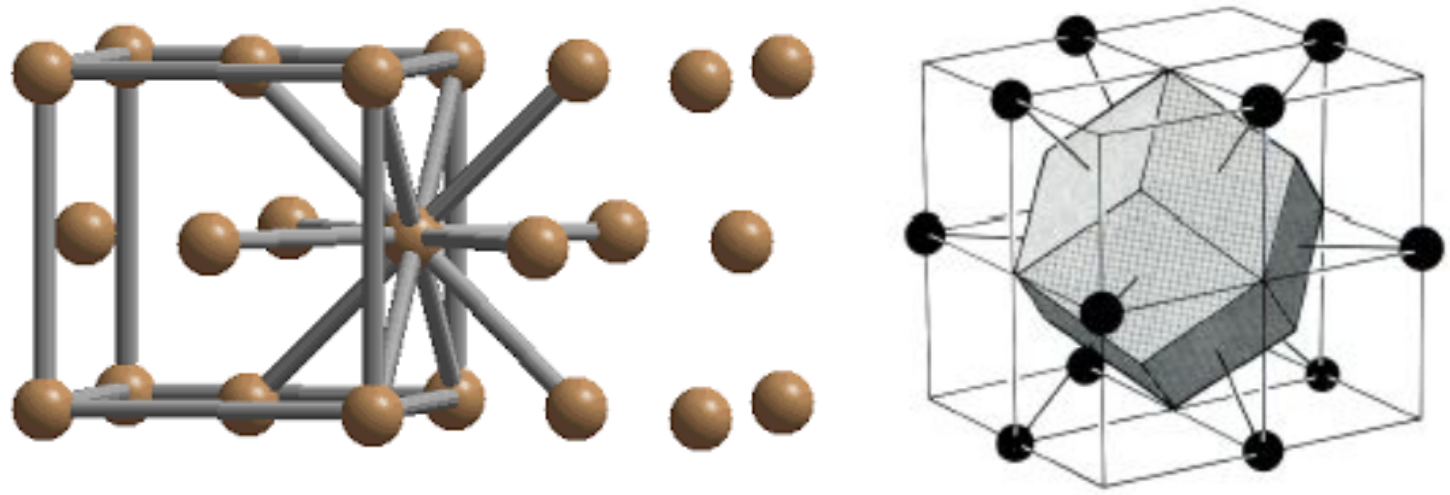
\includegraphics[width=0.7\linewidth]{fig/fcc_wignerseitz.png}
\caption{A rede FCC tem 12 primeiros vizinhos. Sua célula unitária de Wigner-Seitz é um \textit{rhombic dodecahedron}.}
\label{fig:fcc_wignerseitz}
\end{figure}

\begin{itemize}
\item Rotações $C_4$ (nos eixos que ligam aos primeiros vizinhos).
\item Rotações $C_3$ (nos eixos que passam por vértices que incidem 3 arestas)
\item Rotações $C_2$ (nos eixos que passam por pontos médios de arestas).
\item Reflexões em diversos planos do tipo $\sigma_v$ e $\sigma_d$.
\item Identidade e Inversão.
\end{itemize}

\end{frame}


%%%%%%%%%%%%%%%%%%%%%%%%%%%%%%%%%%%%%%%%%%%%%%%%%%%%%%%%%


\begin{frame}{(b) Zonas de Brillouin da rede hexagonal}

As zonas de Brillouin podem ser construídas através da identificação dos planos de Bragg e do número mínimo de cruzamentos realizados por esses planos.

\n

Tome um ponto $\k$ qualquer do espaço recíproco. Considere os caminhos que saem da origem e vão até o ponto $\k$. Se o número mínimo de cruzamentos por planos de Bragg for $n$, então o ponto $\k$ pertence à $(n+1)-$ésima zona de Brillouin.

\begin{figure}[H]
\centering
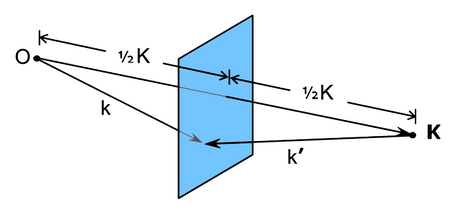
\includegraphics[width=0.35\linewidth]{fig/bragg-plane.png}
\caption{Dado um vetor da rede recíproca $\vb{K}$, o plano de Bragg correspondente é definido como os pontos equidistantes da origem $\vb{O}$ e $\vb{K}$.}
\label{fig:bragg-plane}
\end{figure}

As animações a seguir foram retiradas deste \href{https://www.doitpoms.ac.uk/tlplib/brillouin_zones/zone_construction.php}{\color{blue}{website}}.

\end{frame}


%%%%%%%%%%%%%%%%%%%%%%%%%%%%%%%%%%%%%%%%%%%%%%%%%%%%%%%%%


\begin{frame}{(b) Zonas de Brillouin da rede hexagonal}

\begin{figure}[H]
\centering
\begin{subfigure}{.45\textwidth}
  \centering
  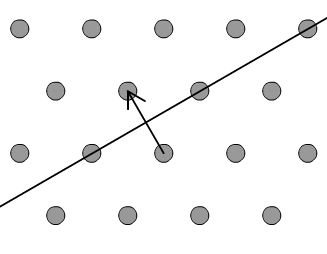
\includegraphics[width=\linewidth]{fig/hexbz_construct-1.png}
\end{subfigure}%
\quad \quad
\begin{subfigure}{.45\textwidth}
  \centering
  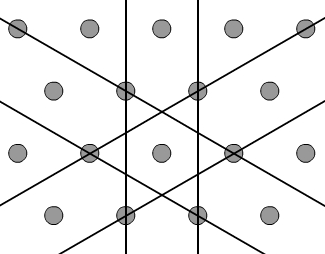
\includegraphics[width=\linewidth]{fig/hexbz_construct-2.png}
\end{subfigure}
\end{figure}

\end{frame}


%%%%%%%%%%%%%%%%%%%%%%%%%%%%%%%%%%%%%%%%%%%%%%%%%%%%%%%%%


\begin{frame}{(b) Zonas de Brillouin da rede hexagonal}

\begin{figure}[H]
\centering
\begin{subfigure}{.45\textwidth}
  \centering
  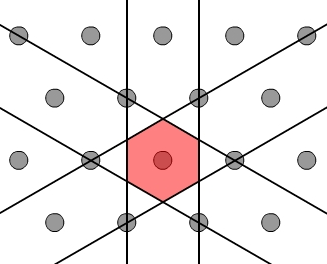
\includegraphics[width=\linewidth]{fig/hexbz_construct-3.png}
\end{subfigure}%
\quad \quad
\begin{subfigure}{.45\textwidth}
  \centering
  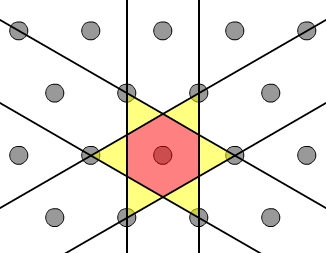
\includegraphics[width=\linewidth]{fig/hexbz_construct-4.png}
\end{subfigure}
\end{figure}

\end{frame}


%%%%%%%%%%%%%%%%%%%%%%%%%%%%%%%%%%%%%%%%%%%%%%%%%%%%%%%%%


\begin{frame}{(b) Zonas de Brillouin da rede hexagonal}

\begin{figure}[H]
\centering
\begin{subfigure}{.45\textwidth}
  \centering
  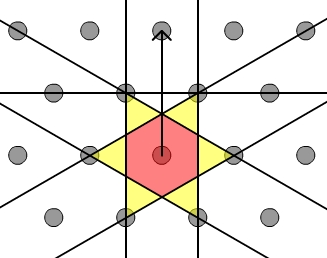
\includegraphics[width=\linewidth]{fig/hexbz_construct-5.png}
\end{subfigure}%
\quad \quad
\begin{subfigure}{.45\textwidth}
  \centering
  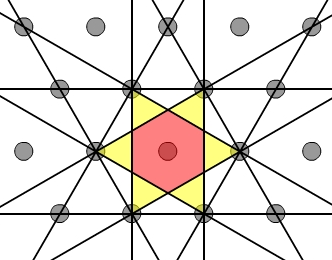
\includegraphics[width=\linewidth]{fig/hexbz_construct-6.png}
\end{subfigure}
\end{figure}

\end{frame}


%%%%%%%%%%%%%%%%%%%%%%%%%%%%%%%%%%%%%%%%%%%%%%%%%%%%%%%%%


\begin{frame}{(b) Zonas de Brillouin da rede hexagonal}

\begin{figure}[H]
\centering
\begin{subfigure}{.45\textwidth}
  \centering
  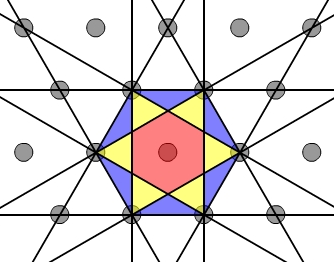
\includegraphics[width=\linewidth]{fig/hexbz_construct-7.png}
\end{subfigure}%
\quad \quad
\begin{subfigure}{.45\textwidth}
  \centering
  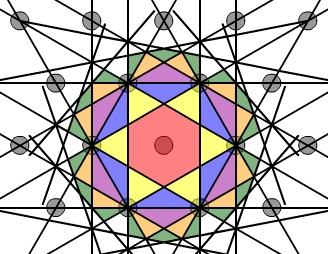
\includegraphics[width=\linewidth]{fig/hexbz_construct-8.png}
\end{subfigure}
\end{figure}

O ``folding'' das zonas de Brillouin pode ser melhor visualizado no link

\textcolor{blue}{\url{https://www.doitpoms.ac.uk/tlplib/brillouin_zones/folding.php}}

\end{frame}


%%%%%%%%%%%%%%%%%%%%%%%%%%%%%%%%%%%%%%%%%%%%%%%%%%%%%%%%%


\begin{frame}{Anotações para a apresentação}

Espaçar mais os slides e destacar os pontos importantes, seja colorindo ou deixando num \text{boxed}.

Relembrar rapidamente o que é uma rede de Bravais.

Explicar o $\a_3 = (0, 0, 1)$.

Desenhar os vetores $\a_1$ e $\a_2$ da rede hexagonal (Figura \ref{fig:lat-triang}).

Mencionar que a reflexão $\sigma_h$ é equivalente à uma rotação $C_2$ com o mesmo eixo da reflexão.

Levar o cubo mágico para a sala e explicar a rotação \textit{2-fold}.

Retirar o cubo preto da Figura \ref{fig:reflex_cubic}, e explicar que o cubo tem outros planos de reflexão.

Fazer no papel o ``folding'' das segunda e terceira zonas de Brillouin e indicar nas figuras.

Citar todos os websites de onde eu tirei as minhas figuras.

\end{frame}


\end{document}
